\documentclass[a4paper]{article}

\usepackage{hyperref}
\hypersetup{
colorlinks=false, % bool: Liens colorés
pdfborder={0 0 0} % Ne pas encadrer les liens
}
\usepackage[utf8]{inputenc}
\usepackage[francais]{babel}
\usepackage[top=2cm, bottom=2cm, left=2cm, right=2cm]{geometry}
\usepackage{graphicx}
\usepackage[final]{pdfpages}
\usepackage{rotating}
\usepackage{eurosym}
\usepackage{lscape}
\usepackage{float}
\usepackage{color}
\usepackage{colortbl}
% définir les commandes ici
\newcommand{\titlecolor}[1]{\textcolor{blue}{\section{#1}}}
\newcommand{\subtitlecolor}[1]{\textcolor[rgb]{0.50,0.50,1.00}{#1}}
% s'il y a beaucoup de commandes et de packages à inclure n'h&ésitez pas
% à mettre tout ça dans un fichier include.tex et l'inclure
% \input{include.tex}




\begin{document}
\title{PdC 4 : Dossier d'Initialisation}
\author{Elisa ABIDH, Adrien BROCHOT, Julien LEVESY, Armand ROSSIUS}

%------------------------------------- Page de titre
\maketitle
%\begin{titlepage}
%~

%\vfill
%\begin{Large}
%Septembre 2011
%\end{Large}
%\vfill
%\end{titlepage}
%----------------------------------------------------

%--------------------------------- Table des matières
\newpage
\tableofcontents
\newpage
%----------------------------------------------- Plan

\titlecolor{Objet et contexte du projet}
\subsection{Objet du projet}
\paragraph{} Ce projet vise à concevoir plusieurs scénarios permettant d'actualiser les architectures applicative et technique en place de la société Péchiney Electrométallurgie (PEM). Le Comité de Pilotage devra avoir les éléments permettant d'évaluer, comparer et choisir l'un de ces scénarios.
Dans le cadre de cette étude il faudra compléter les informations qui ont été recueillis lors des phases antérieures du schéma directeur en particulier les phases d'analyse de l'existant et d'analyse des besoins fonctionnels. Il sera nécessaire de faire une veille technologique des solutions informatique du marché. 
\subsection{Contexte du projet}
L'étude s'inscrit dans le cadre du projet d'élaboration du schéma directeur des systèmes d'information que la société PEM a engagé récemment pour les cinq prochaines années. La société Pecheney Electrométallurgie a réalisé un premier schéma directeur pour l'informatique dans les années 80 qui a conduit à une rénovation importante de son système d'information. L'architecture actuelle est donc en place depuis plusieurs années, elle couvre les principaux besoins du SI opérationnel de l'entreprise.\\ Les principaux objectifs du nouveau plan directeur sont dans ce contexte les suivants :
\begin{itemize}
\item[•]Maitriser les couts
\item[•]Augmenter sa réactivité vis à vis des fournisseurs
\item[•]Améliorer le pilotage de l'entreprise
\item[•]Améliorer la capacité du système d'information
\item[•]Garantir la pérennité du système informatique
\end{itemize}
\titlecolor{Livrables}
\subsection{Livrables de gestion de projet}
\subsubsection{Dossier d'initialisation}
Le dossier d'initialisation présente l'objet du projet. Ce dossier constitue le fondement de l'organisation de l'équipe. Il définit les rôles et responsabilités de chacun. Il précise les différentes tâches et livrables du projet avec leur description. Il contient le planning et le plan de charge qui détaille le temps prévu pour chaque intervenant sur chaque tâche.
Bien que le plan de charge ne soit jamais respecté exactement, il permet d'identifier les tâches les plus longues et de suivre la consommation du temps de chaque intervenant par sa mise à jour tout au long du projet. Voici le plan du dossier d'initialisation :
\begin{itemize}
\item[•]Objet du projet
\item[•]Livrables attendus
\item[•]Organisation et ressources
\item[•]Activités, tâches et planification
\item[•]Procédures de gestion de projet
\item[•]Analyse des risques
\end{itemize}

\subsection{Dossier de production}
\subsubsection{Document de synthèse}
Il contiendra les informations nécessaire pour présenter au Comité de Pilotage les scénarios retenus : architectures cibles et plans de mise en œuvre. Il contiendra également les informations permettant l'évaluation, la comparaison et le choix d'un scénario par le Comité.
\subsubsection{Document d'annexes}
Ce document apportera les éclairages de la synthèse. 
\subsubsection{Document de synthèse de la veille technologique}
Ce document présentera une synthèse de la veille des solutions d'aide au pilotage décisionnel.
\begin{itemize}
\item[•]Définition des solutions de pilotage décisionnel
\item[•]Présentation des solutions existantes 
\end{itemize}

\titlecolor{Organisation et ressources}
\subsection{Ressources}
L'équipe se compose de 4 personnes : Elsia Abidh, qui tiendra le rôle de chef de projet, et Adrien Brochot, Julien Levesy, Armand Rossius qui composeront le groupe d'étude chargé d'élaborer les scénarios.
\subsection{Outils de communication utilisés}
En dehors de réunions et revues, un certain nombre d'outils seront utilisés pour assurer la communication au sein de l'équipe.

\subsubsection{Mails}
Les mails seront utilisés principalement pour fixer des réunions et transmettre des documents entre les membres de l'équipe. Les discussions et débats devront quant à eux être réalisés en face à face. Le chef de projet pourra également communiquer par mail pour demander des corrections sur des résultats, rappeler des objectifs, des dates limites ou des tâches à venir quand le besoin s'en fera sentir trop loin d'une séance de travail en commun, ou sur demande d'un membre de l'équipe.

\subsubsection{Dossier Google Docs}
Un dossier partagé Google Docs a été créé. Il est accessible par tous les membres de l'équipe, et sert à la réflexion et à la transmission de documents. Les documents qu'il contient sont des brouillons ou des notes de réflexion. On ne pourra pas considérer les documents contenus dans ce dossier comme finaux, au moins dans la forme.

\subsection{Outils de travail}
La mise en page finale des documents, une fois l'équipe d'accord sur le fond effectué grâce à Latex. 
Tous les documents devront utiliser le même style, défini par
le chef de projet (en l'absence de Responsable Qualité sur ce projet, compte tenu de la petite taille de l'équipe). La présentation orale sera faite sous Keynote, un logiciel sous mac.
\newpage
\titlecolor{Activités, tâches et planification}

\begin{figure}[!h]
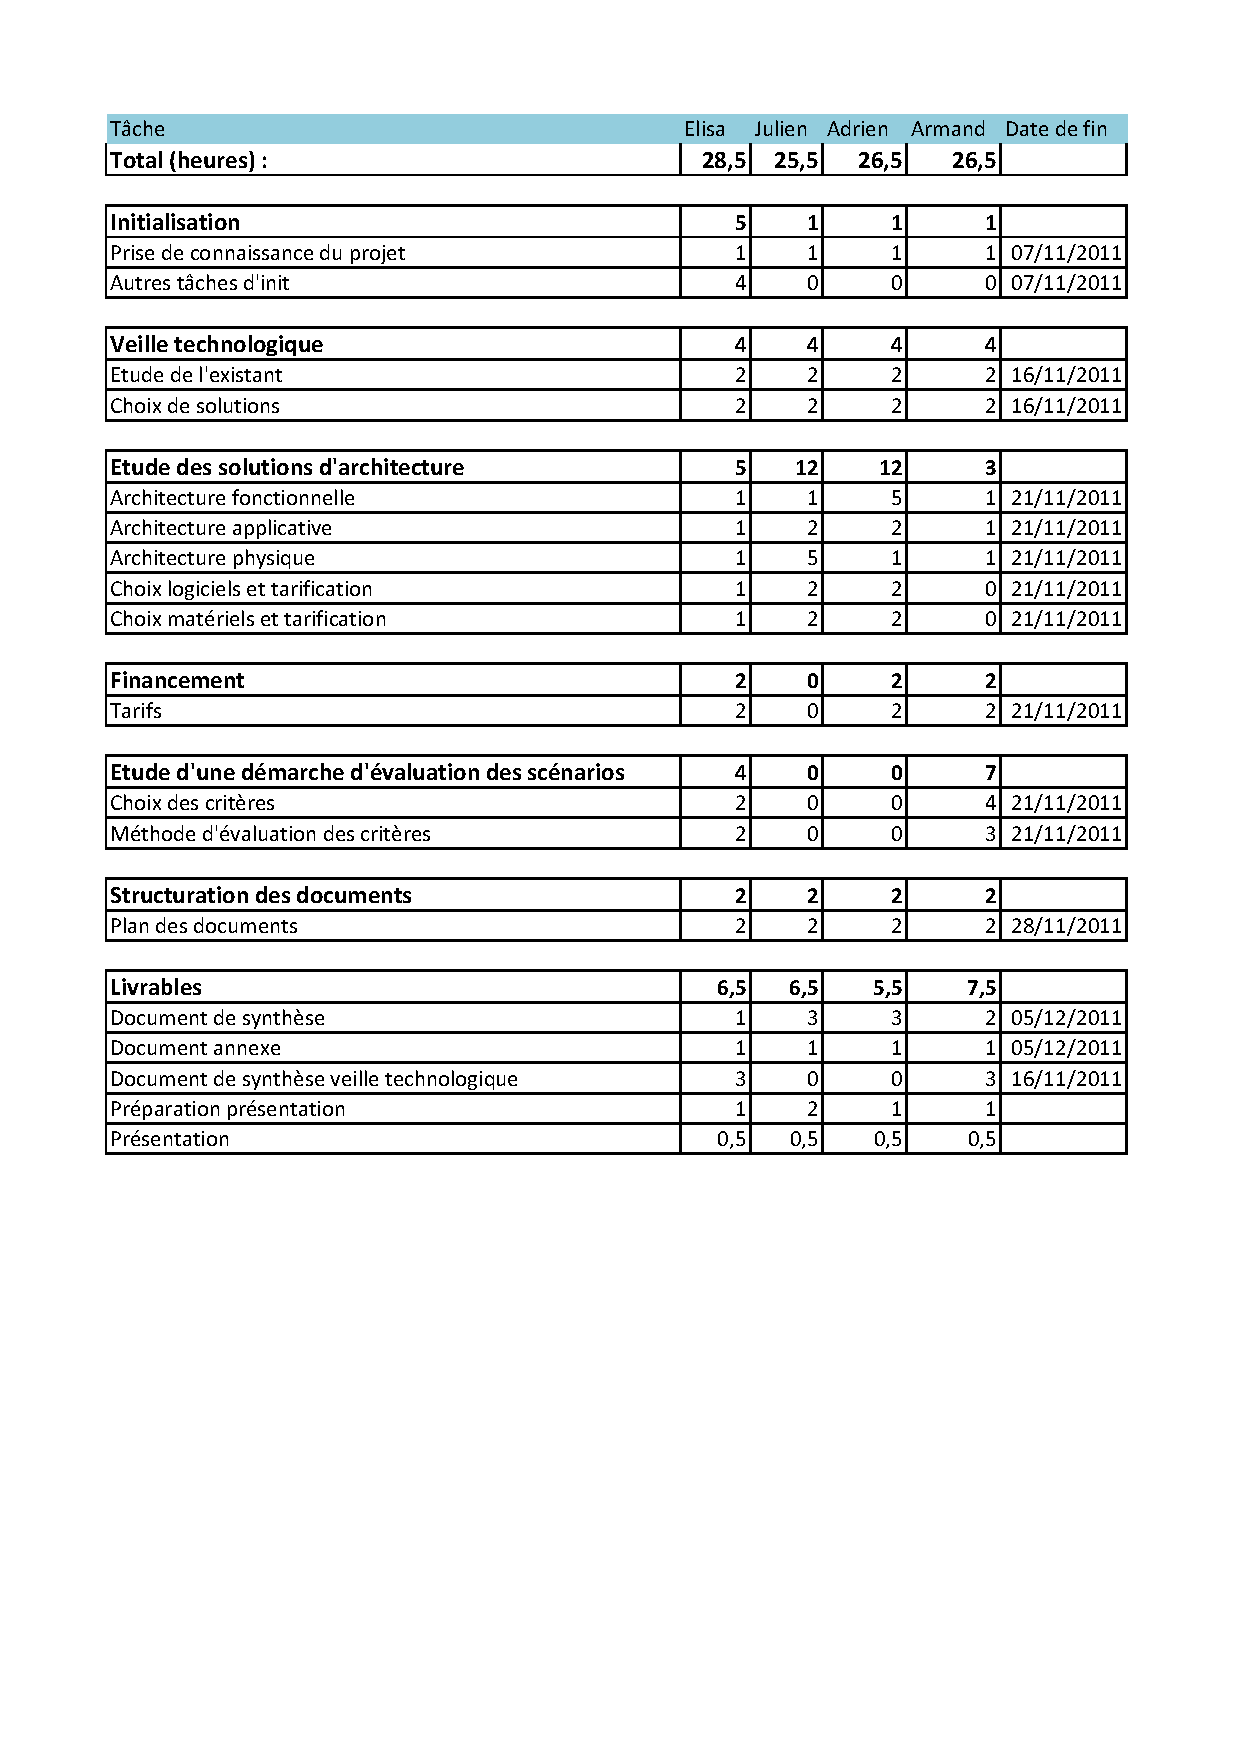
\includepdf [scale= 0.75] {Taches.pdf}
\end{figure}

Le diagramme prévisionnel de Gantt est en annexe 1
\newpage
\titlecolor{Procédures de gestion de projet}
Une revue sera effectuée pendant chaque séance de travail planifiée à l'emploi du temps. Compte tenu de la courte durée de ces séances (2h), et en fonction de l'avancement du projet et de la date de la dernière revue, le chef de projet choisira de la faire au début ou à la fin de la séance. Cette revue permettra de faire un point oral sur l'avancement des tâches, de discuter d'éventuelles questions sur le projet, et de démarrer les nouvelles tâches. Elle servira également à préciser oralement ce qui devra être réalisé d'ici la prochaine séance de travail. Au besoin des réunions exceptionnelles pourront être décidées par le chef de projet entre deux séances de travail, avec toute ou partie de l'équipe. Les membres de l'équipe sont libres d'organiser leur temps de travail à leur souhait, les délais de fin des tâches ayant été fixés à l'avance, ils devront être respectés aux maximum.\\
Dès qu'un membre de l'équipe considère avoir terminé une de ces tâches, il doit prévenir le chef de projet qui validera alors le résultat de ce travail. Si un problème est trouvé, il sera corrigé par l'intervenant ayant réalisé le travail compte tenu du faible nombre de ressources dans le projet. Dès qu'un livrable est considéré comme complet par son rédacteur, qu'il soit le chef de projet ou un autre membre de l'équipe, il devra être relu par un autre membre de l'équipe pour détecter les erreurs de fond, les incohérences, mais également pour corriger les erreurs de forme, les fautes d'orthographe et les soucis de mise en page. Une fois le livrable relu, il sera validé par le chef de projet et pourra alors être présenter lors de la revue avec l'enseignant. Une fois tous les livrables validés par le chef de projet, ils pourront être livrés au client, sous forme numérique en un seul envoi groupé.\\

\titlecolor{Analyse des risques}
Afin d'essayer de prévoir les incidents qui pourraient empêcher le bon déroulement du projet et surtout de les éviter au maximum, nous listerons ci-dessous les risques identifiés.

\newpage
%\begin{figure}[!h]
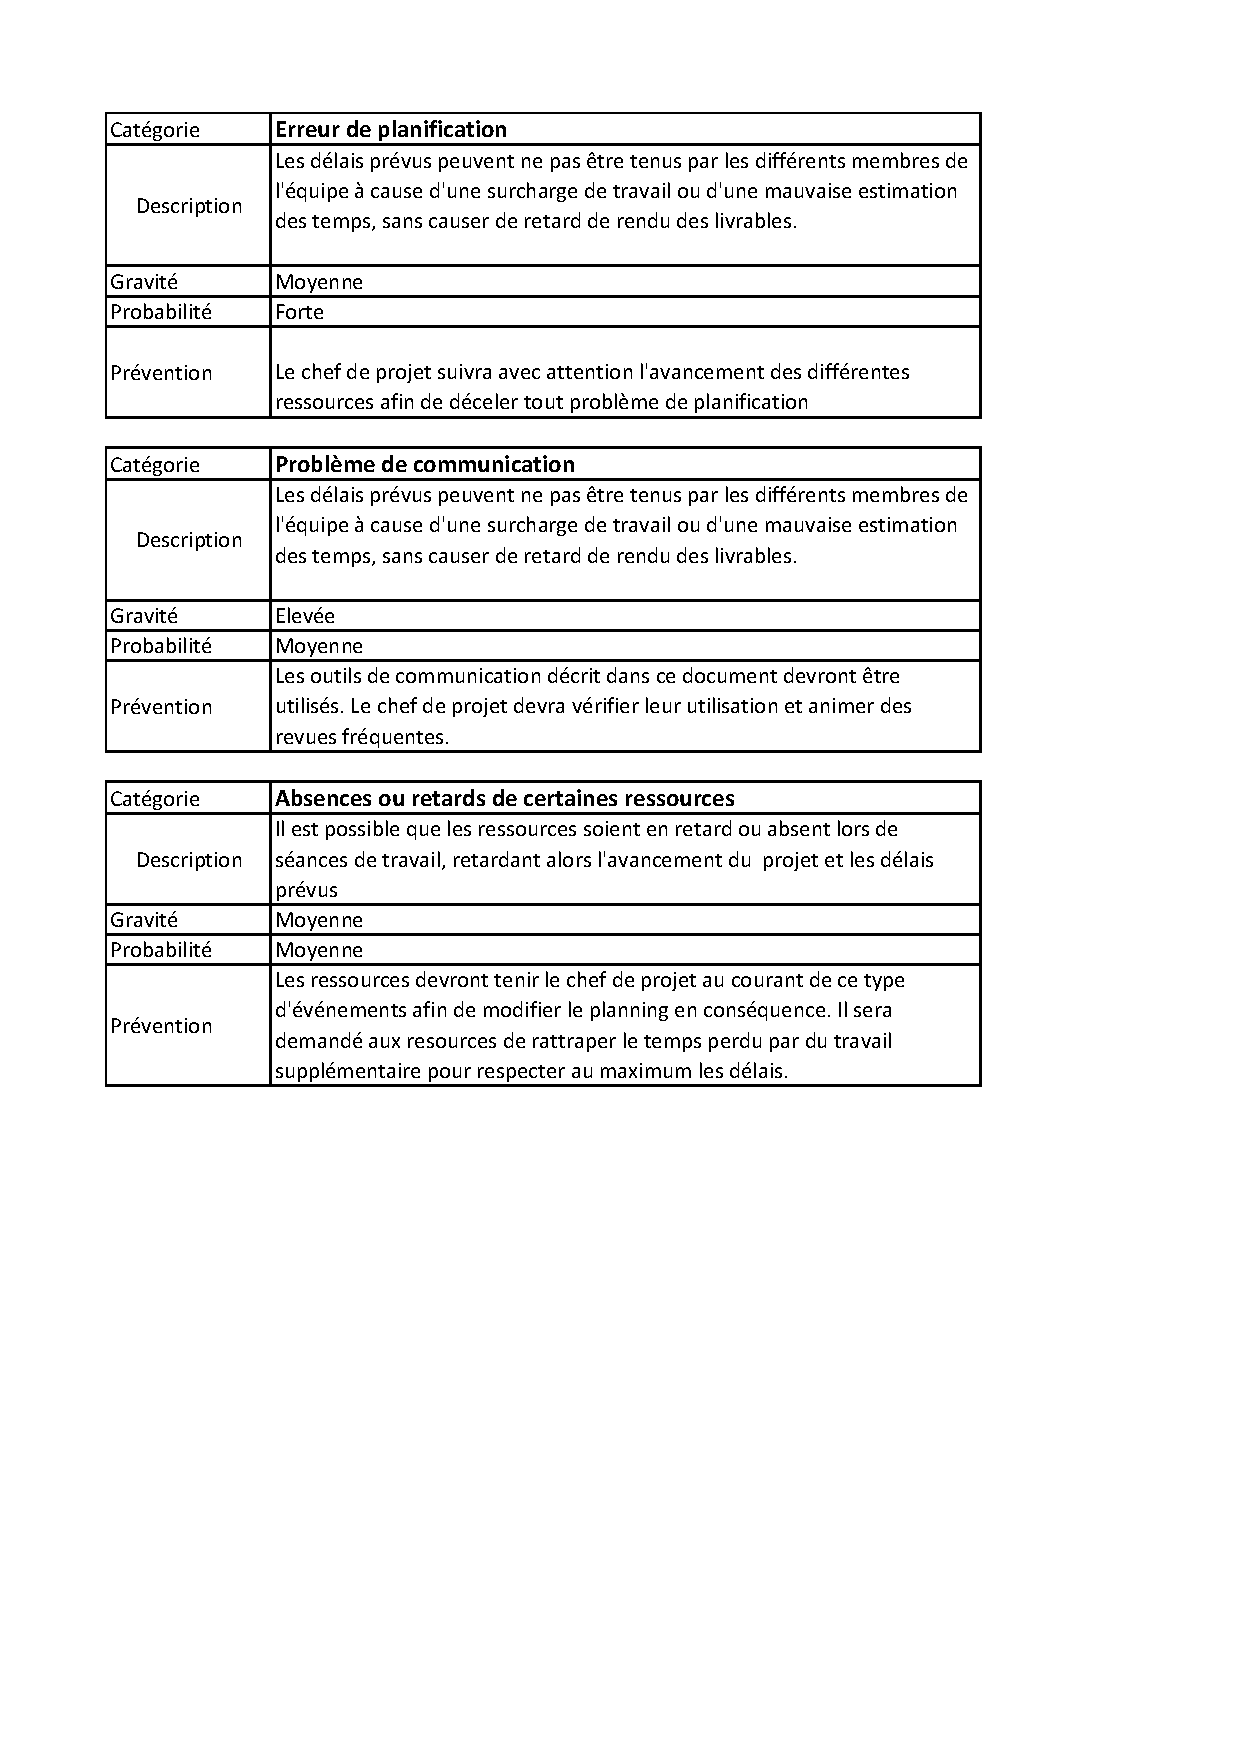
\includepdf [scale= 0.8] {Risques.pdf}
%\end{figure}
\titlecolor{Annexe}
\subsection{Diagramme de Gantt prévisionnel}

\begin{figure}[!h]
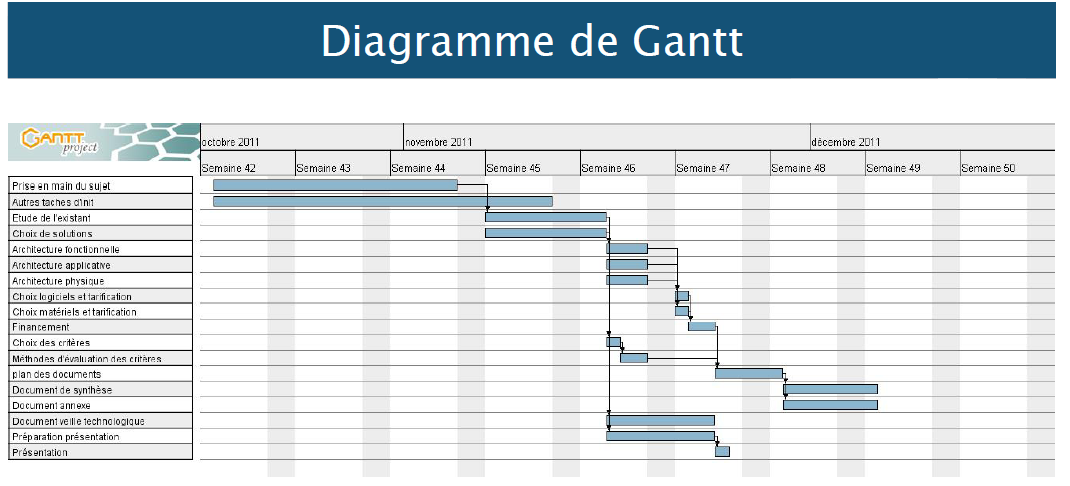
\includegraphics[scale=0.7,angle=90]{gantt.png}
\end{figure}



\end{document}
